\documentclass[11pt,letterpaper]{article}

\usepackage[utf8]{inputenc}
\usepackage[T1]{fontenc}
\usepackage{lmodern}
\usepackage[margin=1in]{geometry}
\usepackage{amsmath,amssymb,amsthm}
\usepackage{graphicx}
\graphicspath{{../}}
\usepackage{booktabs}
\usepackage{siunitx}
\usepackage{hyperref}
\usepackage[numbers]{natbib}
\usepackage{microtype}
\usepackage{newtxtext,newtxmath}
\usepackage{caption}
\usepackage[section]{placeins}

\hypersetup{%
  colorlinks=true,
  linkcolor=blue!50!black,
  citecolor=blue!50!black,
  urlcolor=blue!50!black,
}

\captionsetup[table]{skip=6pt}

% --- float placement tuning: keep figures near their declaration ---
\setcounter{topnumber}{3}
\setcounter{bottomnumber}{2}
\setcounter{totalnumber}{5}
\renewcommand{\topfraction}{0.9}
\renewcommand{\bottomfraction}{0.8}
\renewcommand{\textfraction}{0.07}
\renewcommand{\floatpagefraction}{0.7}

\title{Controller Design for Flapping Flight}
\author{Jean Pecquet}
\date{\today}

\begin{document}
\maketitle
\tableofcontents

\newpage

\section{Introduction}\label{sec:intro}

We propose a control strategy for flapping flight.

\section{Model Description}\label{sec:model}

The lift and drag coefficients are defined as
\begin{align}
    C_L &= C_{L,0} \sin 2\alpha \label{eq:cl} \\
    C_D &= C_{D,0} \cos^2 \alpha + C_{D,\frac{\pi}{2}} \sin^2 \alpha \label{eq:cd}
\end{align}
We denote the nondimensional phase as $\tau^* = \omega^* t^*$.
A wingbeat cycle occurs between $\tau^* = 0$
and $\tau^* = 2\pi$. The flapping kinematics are
\begin{align}
    s^*(\tau^*) = s_0^* \sin\tau^*
\end{align}
The pitch kinematics are
\begin{align}
    \psi(\tau^*) = \psi_0 + \psi_1 \sin(\tau^* - \delta_0)
\end{align}

\section{Controller Design}\label{sec:design}

\subsection{Problem Statement}\label{sec:problem-statement}

We wish to design a control strategy to achieve
arbitrary trajectories in the two-dimensional plane,
including prey pursuit trajectories. We assume that
the flyer's own state is known using a variety
of sensory inputs, so position and velocity are
available as inputs to the controller. In addition,
when a prey is present in the environment,
the bearing angle to the prey, as detected by the eyes,
is also an available input. Because we are
particularly interested in \emph{dragonfly}
flight, we make two design decisions such that the resulting
flight characteristics resemble those of a dragonfly.
First, hovering should be achieved with an inclined stroke
plane (tilted from the horizontal), characterized by
the parameter $\gamma^\text{hover}$. Second, when at speed, the
stroke-plane normal should be approximately aligned
with the direction of travel, as observed in experiments
\cite{azuma1985}. This last choice will simplify
the analysis to follow, since any flow velocity
component parallel to the stroke plane can be neglected.
With these choices in mind, the contents of this section
otherwise hold for flapping flight in general, as we
do not assume specific morphological characteristics
like number of wing pairs, size, etc.

\subsection{Mean Aerodynamic Force}

\subsubsection{Definitions and Assumptions}

To affect its trajectory, the flapping flyer
must modulate and direct the aerodynamic force
acting on its wings. Because the aerodynamic force
on a flapping wing is by nature highly unsteady,
it is convenient to consider the wingbeat-cycle average
of the aerodynamic force, summed over each of the wings,
which we call the \emph{mean aerodynamic force}, $\langle \vec{F}^* \rangle$.
$\langle \vec{F}^* \rangle$ is a function of morphology and wing kinematics,
as well as the flow characteristics in the body frame (this
involves the body kinematics in the fixed frame, as well as
any wind in the fixed frame; in the following we refer
to this simply as the body kinematics, or body velocity,
with the implication that it is relative to the air, which
need not be the same as the fixed frame if there is any wind).
Body velocity is not constant over a wingbeat cycle: there
are (a) oscillations inherent to flapping, and there may be
(b) a net change in body velocity over the cycle.
Assuming the oscillations are small compared to the characteristic
wing velocity, and that any body velocity changes
occur at a slow rate relative to the wingbeat period, the body
velocity may be considered constant over a wingbeat cycle.
The following assumes these conditions are met.
Our objective is now to understand how $\langle \vec{F}^* \rangle$
depends on the wing kinematics at any given body velocity,
so that we are able to formulate a control strategy.

As explained in \autoref{sec:problem-statement}, we
are designing a controller under the assumption that the body velocity
is normal to the stroke plane. Beyond morphology and kinematics,
then, there is a single body velocity parameter $\langle u^* \rangle$,
which is the cycle-averaged body velocity magnitude (the direction
being set to the stroke-plane normal $\hat{n}$).
It is convenient to introduce a similarity parameter in
the form of the \emph{advance ratio}, $J$, which is the
ratio of the cycle-averaged body velocity to the
characteristic wing velocity:
\begin{align}
    J = \frac{\langle u^* \rangle}{s_0^* \omega^*}
\end{align}
The instantaneous wing velocity $\vec{v}^*$
relative to the air has the stroke-plane normal and
in-plane components
\begin{align}
    v_n^* &= \langle u^* \rangle = s_0^* \omega^* J \\
    v_s^* &= s_0^* \omega^* \cos\tau^*
\end{align}
The squared norm of the velocity is
\begin{align}
    (v^*)^2 &= \left(s_0^* \omega^*\right)^2 \left[ J^2 + \cos^2\tau^* \right]\label{eq:v_sq}
\end{align}
We introduce the signed angle $\chi$ from
$\hat{n}$ to $\vec{v}^*$, defined as
\begin{align}
    \chi = -\tan^{-1} \frac{v_s^*}{v_n^*} = -\tan^{-1} \frac{\cos\tau^*}{J}
\end{align}
When $\cos\tau^* > 0$ (stroke along $+\hat{s}$, $\chi < 0$), the angle of attack $\alpha$ is 
\begin{align}
    \alpha = \psi - \chi = \psi + \tan^{-1} \frac{\cos\tau^*}{J}
\end{align}
When $\cos\tau^* < 0$ (stroke along $-\hat{s}$, $\chi > 0$), the angle of attack $\alpha$ is 
\begin{align}
    \alpha = \chi - \psi = -\psi - \tan^{-1} \frac{\cos\tau^*}{J}
\end{align}
The general expression is, then,
\begin{align}
    \alpha = \frac{\cos\tau^*}{|\cos\tau^*|} \psi + \tan^{-1} \frac{|\cos\tau^*|}{J} \label{eq:alpha}
\end{align}
The above is sufficient to obtain the mean
aerodynamic force. The derivation is
somewhat involved in the general case.
We first present the hovering case, which
corresponds to $J = 0$.

\subsubsection{Hover Case $(J=0)$}

For $J=0$, the angle of attack simplifies to
\begin{align}
    \alpha = \frac{\cos\tau^*}{|\cos\tau^*|} \psi + \frac{\pi}{2}
\end{align}
Using the appropriate trigonometric identities, the
aerodynamic coefficients (defined in \autoref{eq:cl} and \autoref{eq:cd})
are
\begin{align}
    C_L &= -\frac{\cos\tau^*}{|\cos\tau^*|} C_{L,0} \sin 2\psi \label{eq:cl-hover} \\
    C_D &= \frac{C_{D,\frac{\pi}{2}} + C_{D,0}}{2} + \frac{C_{D,\frac{\pi}{2}} - C_{D,0}}{2} \cos 2\psi \label{eq:cd-hover}
\end{align}
Because the wing velocity relative to the air
is purely in-plane (along $\hat{s}$), the in-plane aerodynamic force
component is purely drag, and the out-of-plane
component (along $\hat{n}$) is purely lift. The mean
aerodynamic force components are
\begin{align}
    \langle F_n^* \rangle &= \frac12 \frac{A^*}{m^*} \left( s_0^* \omega^* \right)^2 \langle C_L |\cos \tau^*|^2 \rangle \nonumber \\
    &= -\frac12 \frac{A^*}{m^*} \left( s_0^* \omega^* \right)^2 C_{L,0} \langle \sin 2\psi\; \cos \tau^* |\cos \tau^*| \rangle \\
    \langle F_s^* \rangle &= -\frac12 \frac{A^*}{m^*} \left( s_0^* \omega^* \right)^2 \langle C_D \cos \tau^* |\cos \tau^*| \rangle \nonumber \\
    &= -\frac12 \frac{A^*}{m^*} \left( s_0^* \omega^* \right)^2 \frac{C_{D,\frac\pi2} - C_{D,0}}{2}\, \langle \cos 2\psi\; \cos \tau^* |\cos \tau^*| \rangle
\end{align}
Note the constant drag term vanishes because
$\langle \cos \tau^* |\cos \tau^*| \rangle = 0$.
We introduce the shorthand $\Delta C_D = C_{D,\frac\pi2} - C_{D,0}$.
The expressions feature a common pre-factor
we call $q^*$, defined as
\begin{align}
    q^* = \frac14 \frac{A^*}{m^*} \left( s_0^* \omega^* \right)^2\label{eq:q}
\end{align}
We further introduce the normal and in-plane force
coefficients $C_{F^*_n}$ and $C_{F^*_s}$, defined as
\begin{align}
    C_{F^*_n} &= \frac{F^*_n}{q^*} = -2 C_{L,0} \langle \sin 2\psi\; \cos \tau^* |\cos \tau^*| \rangle \label{eq:cfn} \\
    C_{F^*_s} &= \frac{F^*_s}{q^*} = -\Delta C_D \langle \cos 2\psi\; \cos \tau^* |\cos \tau^*| \rangle \label{eq:cfs}
\end{align}
which we synthesize into the overall force magnitude coefficient
\begin{align}
    C_{F^*} = \sqrt{C_{F^*_n}^2 + C_{F^*_s}^2}
\end{align}
This coefficient is useful because it is only
a function of the pitch kinematic parameters and the lift
and drag coefficient parameters, and is independent
of morphology and wingbeat frequency and amplitude, which appear
only in the pre-factor $q^*$. 
By maximizing the value of this coefficient,
given a constraint on the force direction
required to achieve a given maneuver,
the characteristic wingbeat velocity $s_0^* \omega^*$ can be minimized.
With our parametrization
of the pitch kinematics, and with the lift
and drag coefficient parameters set, $C_{F^*}$
and its $(n,s)$ decomposition are functions
of 3 variables: $\psi_0$, $\psi_1$, and $\delta_0$.
We visualize $C_{F^*}$, $C_{F^*_n}$, and $C_{F^*_s}$
across slices of this 3D space in \autoref{fig:cf_components}
and \autoref{fig:cf}.
\begin{figure}[htbp]
    \centering
    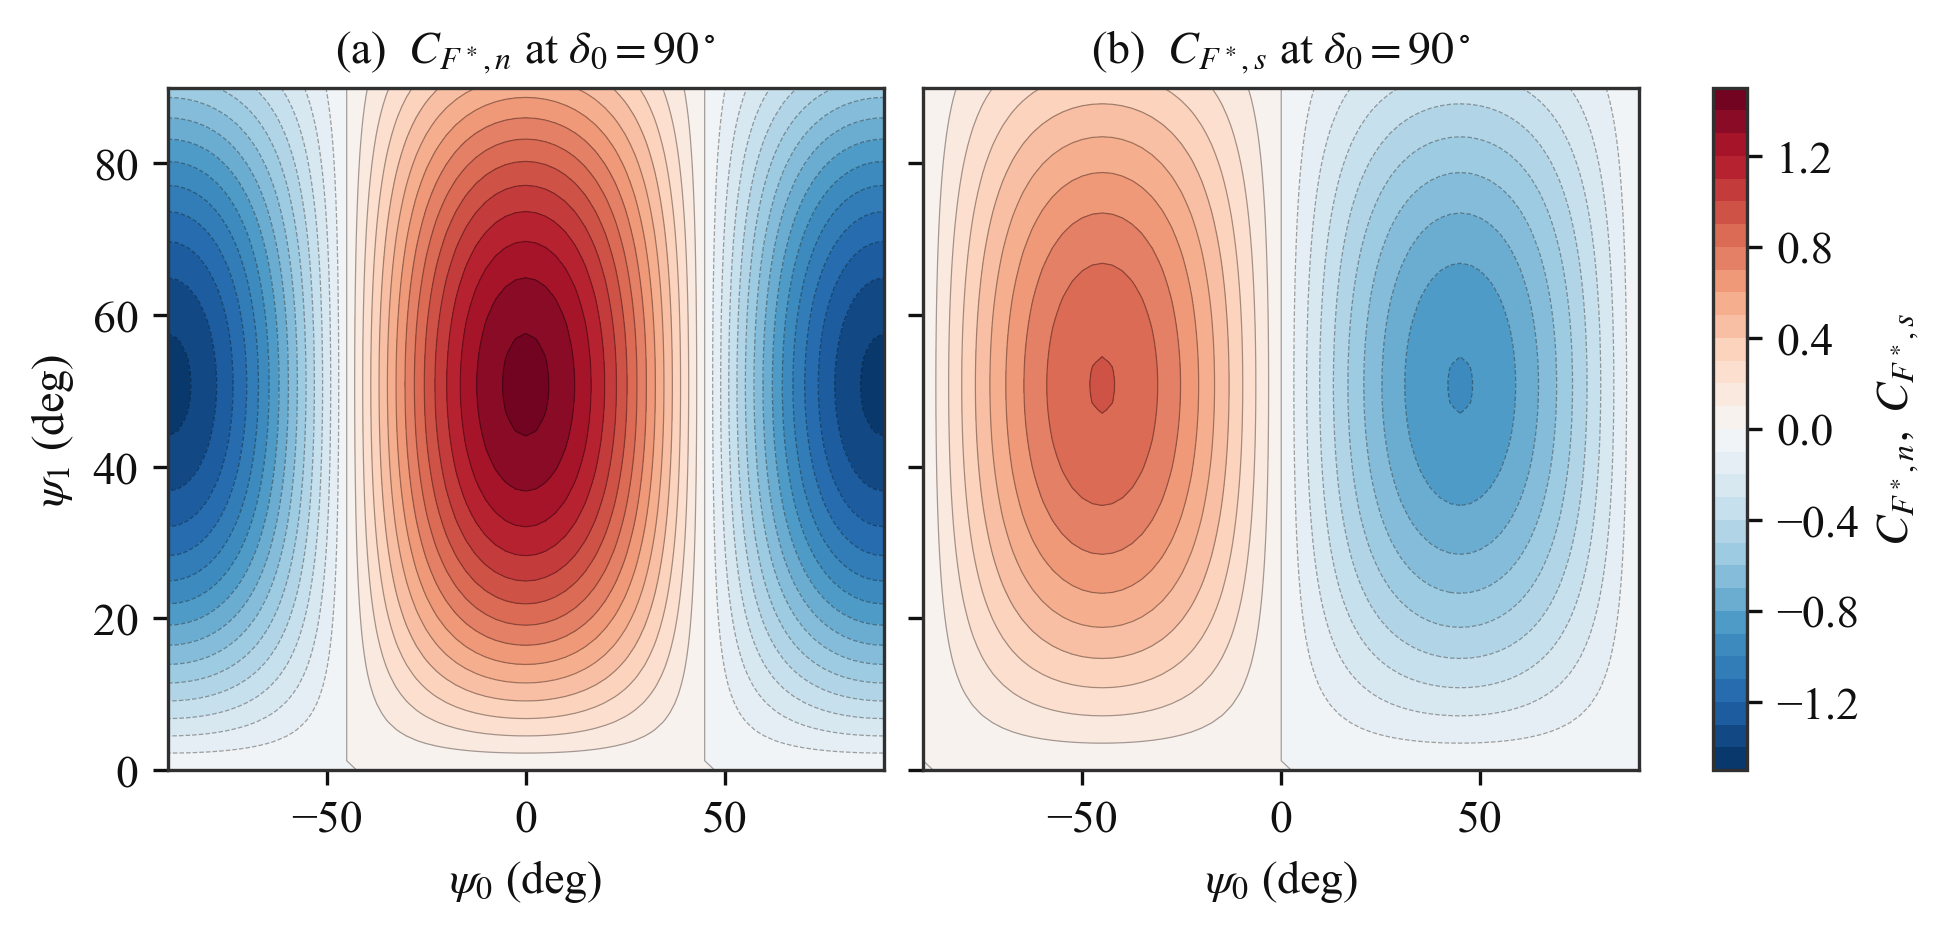
\includegraphics{figures/cf_components.light.png}
    \caption{(a) Stroke-plane-normal (lift) component $C_{F^*_n}$ and
    (b) in-plane (drag) component $C_{F^*_s}$ of the force coefficient
    over the pitch plane at $\delta_0 = 90^\circ$. The force direction
quadrant in the $(\hat{s},\hat{n})$ plane can be inferred from the signs.}\label{fig:cf_components}
\end{figure}
\begin{figure}[htbp]
    \centering
    
\includegraphics{figures/pitch_efficiency.light.png}
    \caption{Dependence of $C_{F^*}$ on pitch parameters at zero body velocity. Maximum shown as white dots.}\label{fig:cf}
\end{figure}

As panel (a) of \autoref{fig:cf} makes evident,
significantly more force is produced when
$\delta_0 = \pm90^\circ$. Because $\delta_0 = -90^\circ$
results in the mean force pointing along $-\hat{n}$
when the mean pitch is neutral ($\psi_0 = 0^\circ$),
we select $\delta_0 = +90^\circ$ as the operating point.
This choice maximizes the mean force for a given
$(\psi_0, \psi_1)$, and reduces the pitch parameter space to 2D.
How then do we select $\psi_0$ and $\psi_1$? It is
clear from panel (b) that a certain value of $\psi_1$,
around $\psi_1 \approx 50^\circ$,
maximizes $C_{F^*}$ for any given $\psi_0$.
We will call it $\psi_1^\text{opt}$.
In addition, $\psi_0 = 0^\circ\pmod{90^\circ}$
maximizes $C_{F^*}$. Looking at panel (b) of \autoref{fig:cf_components},
it is clear that the in-plane force component is zero when
$\psi_0 = 0^\circ\pmod{90^\circ}$, so the force
is purely normal to the stroke plane. In addition,
from panel (a) of the same figure, we see that $\psi_0 = 0^\circ$
results in the mean force pointing towards $+\hat{n}$,
while $\psi_0 = \pm90^\circ$ results in the mean force
pointing towards $-\hat{n}$. We select neutral pitch
($\psi_0 = 0^\circ$) as the reference,
for consistency with the choice of $\delta_0 = 90^\circ$.
In summary, the reference pitch kinematics
\begin{align}
    \psi_0 = 0^\circ \quad\quad\quad \psi_1 = \psi_1^\text{opt} \quad\quad\quad \delta_0 = 90^\circ
\end{align}
result in $C_{F^*} = C_{F^*}^\text{max}$,
and $\langle \vec{F}^* \rangle$
pointing towards $+\hat{n}$.
These reference kinematics allow for \emph{efficient} hover
(in the sense that the characteristic wingbeat velocity $s_0^* \omega^*$
is minimized, because $C_{F^*}$ is maximized) when the stroke
plane is horizontal ($\gamma^\text{hover} = 0^\circ$). Indeed, since
the mean force vector points towards $+\hat{n}$,
$+\hat{n}$ must be vertical and opposed to the direction
of gravity. To model dragonfly hover specifically,
at an inclined stroke plane ($\gamma^\text{hover} \neq 0^\circ$),
the mean force vector must have an in-plane component.
Looking at panel (b) of \autoref{fig:cf_components},
it is clear that this can be achieved by changing $\psi_0$,
away from the symmetric $0^\circ$ point. For convenience,
we introduce $\beta$, the signed angle from the stroke-plane
normal $\hat{n}$ to the mean force vector. Since the mean force is
$\langle \vec{F}^* \rangle = q^* \left( C_{F^*_n} \hat{n} + C_{F^*_s} \hat{s} \right)$,
$\beta$ can be expressed from the $C_{F^*_n}$ and $C_{F^*_s}$ coefficients
(\autoref{eq:cfn} and \autoref{eq:cfs}) as
\begin{align}
    \beta = -\tan^{-1} \frac{C_{F^*_s}}{C_{F^*_n}}
    = -\tan^{-1} \left[ \frac{\Delta C_D}{2 C_{L,0}}
    \frac{\langle \cos2\psi \cos\tau^* |\cos\tau^*| \rangle}{\langle \sin2\psi \cos\tau^* |\cos\tau^*| \rangle} \right]\label{eq:beta}
\end{align}
We can simplify the $\langle \cos2\psi \cos\tau^* |\cos\tau^*| \rangle / \langle \sin2\psi \cos\tau^* |\cos\tau^*| \rangle$
ratio in the above expression.
With $\delta_0 = 90^\circ$, the pitch kinematics reduce to
$\psi = \psi_0 - \psi_1 \cos\tau^*$. Using the appropriate
trigonometric identities,
\begin{align}
    \cos 2\psi &= \cos 2\psi_0 \cos\left(2\psi_1 \cos\tau^*\right) + \sin 2\psi_0 \sin\left(2\psi_1 \cos\tau^*\right) \\
    \sin 2\psi &= \sin 2\psi_0 \cos\left(2\psi_1 \cos\tau^*\right) - \cos 2\psi_0 \sin\left(2\psi_1 \cos\tau^*\right)
\end{align}
Under the half-period shift $\tau^* \to \tau^* + \pi$, the factors
$\cos\tau^* |\cos\tau^*|$ and $\sin\left(2\psi_1 \cos\tau^*\right)$
change sign while $\cos\left(2\psi_1 \cos\tau^*\right)$ is unchanged,
so the $\cos\left(2\psi_1 \cos\tau^*\right)$ terms average to zero,
leading to
\begin{align}
    \langle \cos2\psi\; \cos\tau^* |\cos\tau^*| \rangle &= \sin 2\psi_0\, \langle \sin\left(2\psi_1 \cos\tau^*\right) \cos\tau^* |\cos\tau^*| \rangle \\
    \langle \sin2\psi\; \cos\tau^* |\cos\tau^*| \rangle &= -\cos 2\psi_0\, \langle \sin\left(2\psi_1 \cos\tau^*\right) \cos\tau^* |\cos\tau^*| \rangle
\end{align}
The common $\langle \sin\left(2\psi_1 \cos\tau^*\right) \cos\tau^* |\cos\tau^*| \rangle$
factor cancels out in the ratio, giving simply
\begin{align}
    \frac{\langle \cos2\psi\; \cos\tau^* |\cos\tau^*| \rangle}{\langle \sin2\psi\; \cos\tau^* |\cos\tau^*| \rangle} = -\tan 2\psi_0
\end{align}
and \autoref{eq:beta} becomes
\begin{align}
    \beta = \tan^{-1} \left[ \frac{\Delta C_D}{2 C_{L,0}} \tan 2\psi_0 \right]\label{eq:beta-hover}
\end{align}
Importantly, $\beta$ is independent of $\psi_1$,
and is only controlled by $\psi_0$. It follows that
$\psi_0$ is an appropriate control variable for
the mean force direction relative to the stroke-plane
normal $\hat{n}$. $\beta$ is shown as a function
of $\psi_0$ in \autoref{fig:beta_vs_psi0}.
As discussed above, $C_{F^*}$ becomes less than
its maximum when $\psi_0 \neq 0^\circ\pmod{90^\circ}$, away
from the reference pitch kinematics, so it is also shown
in addition to $\beta$.
\begin{figure}[htbp]
    \centering
    
\includegraphics{figures/force_direction_test.light.png}
    \caption{Effect of $\psi_0$ on force direction angle $\beta$ and force coefficient $C_{F^*}$.}\label{fig:beta_vs_psi0}
\end{figure}
In the $\Delta C_D / \left( 2 C_{L,0} \right) \to 1$ limit,
the relation between $\beta$ and $\psi_0$
can be approximated as $\beta \approx 2\psi_0$.
This holds only roughly here because 
$\Delta C_D / \left( 2 C_{L,0} \right) = 1.9/3 \approx 0.63$,
but the trend is the same, as can be seen in the figure.
To achieve hover at an inclined stroke plane
with tilt angle $\gamma^\text{hover}$, the mean force vector
angle must be $\beta = -\gamma^\text{hover}$. 
This requires $\psi_0 = \psi_0^\text{hover}$, given
by \autoref{eq:beta-hover} (specifically the inverse
relation) when $\beta = -\gamma^\text{hover}$.

Now that we have narrowed down the pitch
kinematics for hover, we step back to consider
the flapping kinematics as well, governed by
parameters $s_0^*$ (amplitude) and $\omega^*$
(frequency). The condition for hover on the mean
force magnitude is
\begin{align}
    C_{F^*} q^* = 1 \implies (s_0^* \omega^*)^2 = \frac{4}{C_{F^*} \frac{A^*}{m^*}}
\end{align}
We prefer to consider $\omega^*$ as a fixed
parameter rather than a control variable,
leaving $s_0^*$ as the primary control for
the force amplitude. The hover value is given by
\begin{align}
    (s_0^*)^\text{hover} = \frac{1}{\omega^*} \sqrt{\frac{4}{C_{F^*}^\text{hover} \frac{A^*}{m^*}}}
\end{align}
The hover kinematic parameters are summarized in \autoref{tab:hover}.
The control variables are $s_0^*$ and $\psi_0$.
\begin{table}[htbp]
  \centering
  \caption{Wing kinematic parameters for hover}
  \label{tab:hover}
  \begin{tabular}{llr}
    \toprule
    Parameter & Value & Variables \\
    \midrule
    $s_0^*$ & $(s_0^*)^\text{hover}$ & $\frac{A^*}{m^*} \quad \omega^* \quad \gamma^\text{hover} \quad C_{L,0} \quad \Delta C_D$ \\
    $\psi_0$ & $\psi_0^\text{hover}$ & $\gamma^\text{hover} \quad C_{L,0} \quad \Delta C_D$ \\
    $\psi_1$ & $\psi_1^\text{opt}$ & None \\
    $\delta_0$ & $90^\circ$ & None \\
    \bottomrule
  \end{tabular}
\end{table}

\subsubsection{General Case $(J \geq 0)$}

For $J \neq 0$, the wing velocity relative to the air is no longer
purely in-plane, so lift and drag each contribute to both force
components. In terms of the angle $\chi$, the wing velocity direction
is $\hat{v} = \cos\chi\, \hat{n} - \sin\chi\, \hat{s}$. Drag acts
along $-\hat{v}$, and lift acts along the perpendicular direction
\begin{align}
    \hat{\ell} = -\sigma \left( \sin\chi\, \hat{n} + \cos\chi\, \hat{s} \right)
    \quad\quad\quad
    \sigma \equiv \frac{\cos\tau^*}{|\cos\tau^*|}
\end{align}
whose sense alternates between half-strokes, consistent with the sign
convention used to define $\alpha$ (in the hover case, $\hat{\ell}$
reduces to $+\hat{n}$ on both half-strokes). The instantaneous force is
\begin{align}
    \vec{F}^* = \frac12 \frac{A^*}{m^*} (v^*)^2 \left( C_L\, \hat{\ell} - C_D\, \hat{v} \right)
\end{align}
with components
\begin{align}
    F^*_n &= \frac12 \frac{A^*}{m^*} (v^*)^2 \left( -\sigma \sin\chi\; C_L - \cos\chi\; C_D \right) \\
    F^*_s &= -\frac12 \frac{A^*}{m^*} (v^*)^2 \left( \sigma \cos\chi\; C_L - \sin\chi\; C_D \right)
\end{align}
Substituting $\cos\chi = J/\sqrt{J^2 + \cos^2\tau^*}$,
$\sin\chi = -\cos\tau^*/\sqrt{J^2 + \cos^2\tau^*}$, and the expression
for $(v^*)^2$ (\autoref{eq:v_sq}), we get
\begin{align}
    F^*_n &= \frac12 \frac{A^*}{m^*} \left( s_0^* \omega^* \right)^2 \sqrt{J^2 + \cos^2\tau^*}\, \left( |\cos\tau^*|\; C_L - J\; C_D \right) \\
    F^*_s &= -\frac12 \frac{A^*}{m^*} \left( s_0^* \omega^* \right)^2 \sqrt{J^2 + \cos^2\tau^*}\, \left( \sigma J\; C_L + \cos\tau^*\; C_D \right)
\end{align}
Writing $\theta \equiv \tan^{-1} \left( |\cos\tau^*|/J \right)$, such that
$\alpha = \sigma \psi + \theta$ (see \autoref{eq:alpha}),
\begin{align}
    \cos 2\theta = \frac{J^2 - \cos^2\tau^*}{J^2 + \cos^2\tau^*}
    \quad\quad\quad
    \sin 2\theta = \frac{2 J |\cos\tau^*|}{J^2 + \cos^2\tau^*}
\end{align}
and the aerodynamic coefficients (\autoref{eq:cl} and \autoref{eq:cd})
become
\begin{align}
    C_L &= C_{L,0} \left( \sigma \cos2\theta\; \sin2\psi + \sin2\theta\; \cos2\psi \right) \\
    C_D &= \bar{C}_D - \frac{\Delta C_D}{2} \left( \cos2\theta\; \cos2\psi - \sigma \sin2\theta\; \sin2\psi \right)
\end{align}
where we define $\bar{C}_D \equiv \left( C_{D,\frac\pi2} + C_{D,0} \right)/2$
for brevity.
Substituting into the force components, using $\sigma |\cos\tau^*| = \cos\tau^*$
and $\sigma^2 = 1$, and averaging, the force coefficients are
\begin{align}
    C_{F^*_n} &= 2 \left\langle \frac{\left[ C_{L,0} \left( J^2 - \cos^2\tau^* \right) - \Delta C_D\, J^2 \right] \cos\tau^*\, \sin2\psi}{\sqrt{J^2 + \cos^2\tau^*}} \right\rangle \nonumber \\
    &\quad + 2 \left\langle \frac{J \left[ 2 C_{L,0} \cos^2\tau^* + \frac{\Delta C_D}{2} \left( J^2 - \cos^2\tau^* \right) \right] \cos2\psi}{\sqrt{J^2 + \cos^2\tau^*}} \right\rangle
    - 2 J \bar{C}_D \left\langle \sqrt{J^2 + \cos^2\tau^*} \right\rangle \label{eq:cfn-general} \\
    C_{F^*_s} &= -2 \left\langle \frac{J \left[ C_{L,0} \left( J^2 - \cos^2\tau^* \right) + \Delta C_D \cos^2\tau^* \right] \sin2\psi}{\sqrt{J^2 + \cos^2\tau^*}} \right\rangle \nonumber \\
    &\quad - 2 \left\langle \frac{\left[ 2 C_{L,0} J^2 - \frac{\Delta C_D}{2} \left( J^2 - \cos^2\tau^* \right) \right] \cos\tau^*\, \cos2\psi}{\sqrt{J^2 + \cos^2\tau^*}} \right\rangle \label{eq:cfs-general}
\end{align}
Note the constant ($\bar{C}_D$) drag term of $C_{F^*_s}$ vanishes
because $\langle \cos\tau^* \sqrt{J^2 + \cos^2\tau^*} \rangle = 0$.
Setting $J = 0$ recovers \autoref{eq:cfn} and \autoref{eq:cfs},
as expected. At the operating point $\delta_0 = 90^\circ$,
$\psi = \psi_0 - \psi_1 \cos\tau^*$, and the parity argument of the
hover case applies unchanged: under $\tau^* \to \tau^* + \pi$, the
bracketed polynomials and $\sqrt{J^2 + \cos^2\tau^*}$ are invariant,
so expanding $\sin2\psi$ and $\cos2\psi$ and discarding the vanishing
averages leaves
\begin{align}
    C_{F^*_n} &= 2\, I_n(J, \psi_1)\, \cos2\psi_0 - 2 J \bar{C}_D\, I_0(J) \label{eq:cfn-general-op} \\
    C_{F^*_s} &= -2\, I_s(J, \psi_1)\, \sin2\psi_0 \label{eq:cfs-general-op}
\end{align}
with
\begin{align}
    I_0 &= \left\langle \sqrt{J^2 + \cos^2\tau^*} \right\rangle \\
    I_n &= \left\langle \frac{J \left[ 2 C_{L,0} \cos^2\tau^* + \frac{\Delta C_D}{2} \left( J^2 - \cos^2\tau^* \right) \right] \cos\left( 2\psi_1 \cos\tau^* \right)}{\sqrt{J^2 + \cos^2\tau^*}} \right\rangle \nonumber \\
    &\quad - \left\langle \frac{\left[ C_{L,0} \left( J^2 - \cos^2\tau^* \right) - \Delta C_D\, J^2 \right] \cos\tau^*\, \sin\left( 2\psi_1 \cos\tau^* \right)}{\sqrt{J^2 + \cos^2\tau^*}} \right\rangle \\
    I_s &= \left\langle \frac{J \left[ C_{L,0} \left( J^2 - \cos^2\tau^* \right) + \Delta C_D \cos^2\tau^* \right] \cos\left( 2\psi_1 \cos\tau^* \right)}{\sqrt{J^2 + \cos^2\tau^*}} \right\rangle \nonumber \\
    &\quad + \left\langle \frac{\left[ 2 C_{L,0} J^2 - \frac{\Delta C_D}{2} \left( J^2 - \cos^2\tau^* \right) \right] \cos\tau^*\, \sin\left( 2\psi_1 \cos\tau^* \right)}{\sqrt{J^2 + \cos^2\tau^*}} \right\rangle
\end{align}
The angle from the stroke-plane normal to the mean force
(\autoref{eq:beta}) becomes
\begin{align}
    \beta = \tan^{-1} \left[ \frac{I_s \sin2\psi_0}{I_n \cos2\psi_0 - J \bar{C}_D\, I_0} \right] \label{eq:beta-general}
\end{align}
In the limit $J \to 0$, the $I_0$ term vanishes and
\begin{align}
    I_n \to C_{L,0} \left\langle \sin\left( 2\psi_1 \cos\tau^* \right) \cos\tau^* |\cos\tau^*| \right\rangle
    \quad\quad\quad
    I_s \to \frac{\Delta C_D}{2} \left\langle \sin\left( 2\psi_1 \cos\tau^* \right) \cos\tau^* |\cos\tau^*| \right\rangle
\end{align}
recovering \autoref{eq:beta-hover}. The overall force
coefficient $C_{F^*}$ is shown in \autoref{fig:cf_J}
for values of $J$ from 0 to 1, at $\delta_0 = 90^\circ$.
Highlighted on each panel
is the reference point from the hover plot \autoref{fig:cf},
tracked as it turns from a global maximum at $J=0$ to a local
maximum, and eventually to a saddle point.
This point represents the maximum
force available in the $+\hat{n}$ direction for a given $J$.
The region of space within the dotted contour around
the reference point corresponds to $C_{F^*_n} > 0$.
Within this region, the stroke-plane-normal
component of the mean force points towards $+\hat{n}$.

The values of $C_{F^*}$ and $\psi_1$ at the reference point
are shown as functions of $J$ in \autoref{fig:hover_opt_J}.
As the figure makes clear, to obtain the maximum force along
$+\hat{n}$, $\psi_1$ should be decreased as $J$ increases.
The mechanism behind this is illustrated in \autoref{fig:psi1-decrease}.
For a given $\psi$, $\alpha$ decreases as $J$ is increased.
This moves us away from the ideal $\alpha$, reducing lift,
and in turn the force component along $+\hat{n}$.
By decreasing $\psi$, the ideal $\alpha$ is recovered,
thrust along $+\hat{n}$ is maximized. Of course, this is
an instantaneous picture, but the conclusion can be
extended to the mean force over the wingbeat stroke.
To achieve the required reduction in $\psi$
everywhere throughout the stroke, it is hopefully clear that
the relevant parameter is $\psi_1$.
\begin{figure}[htbp]
    \centering
    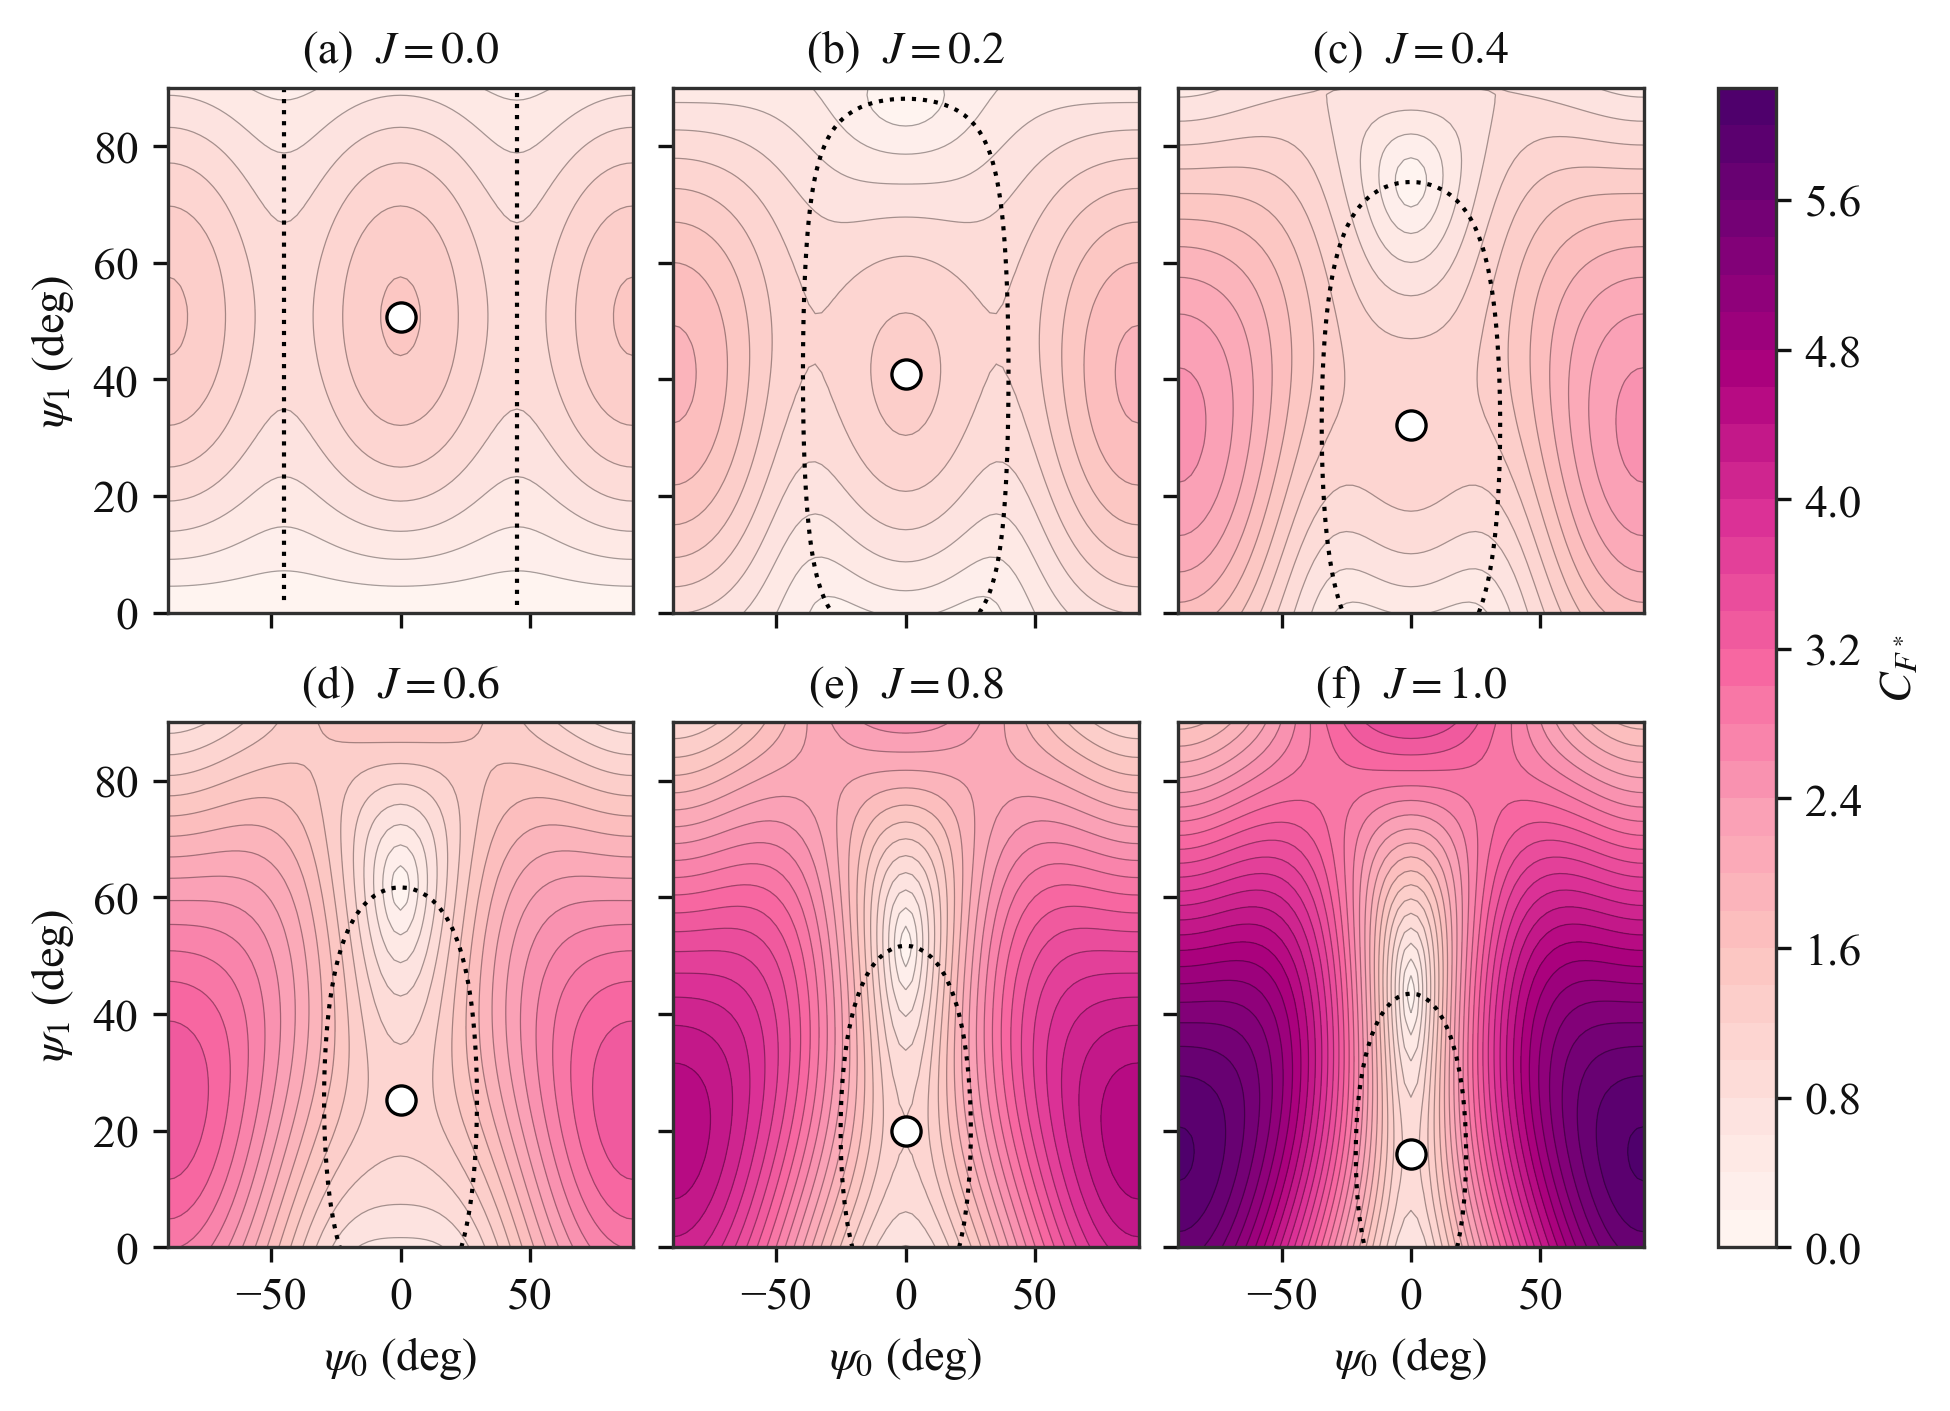
\includegraphics{figures/pitch_efficiency_J.light.png}
    \caption{Force coefficient $C_{F^*}$ over the pitch plane
    $(\psi_0, \psi_1)$ at $\delta_0 = 90^\circ$, for increasing advance
    ratio $J$. White dots track the hover optimum as it moves with $J$.
    It remains on the $\psi_0 = 0^\circ$ axis by symmetry while $\psi_1$
    decreases, and it turns from a local maximum into a saddle point.
    The global maximum sits at large $|\psi_0|$, where the force is
    dominated by drag from the normal inflow and points along
    $-\hat{n}$. The dotted contour marks $C_{F^*_n} = 0$, the boundary
    between propulsive ($+\hat{n}$) and braking ($-\hat{n}$) mean
    force.}\label{fig:cf_J}
\end{figure}
\begin{figure}[htbp]
    \centering
    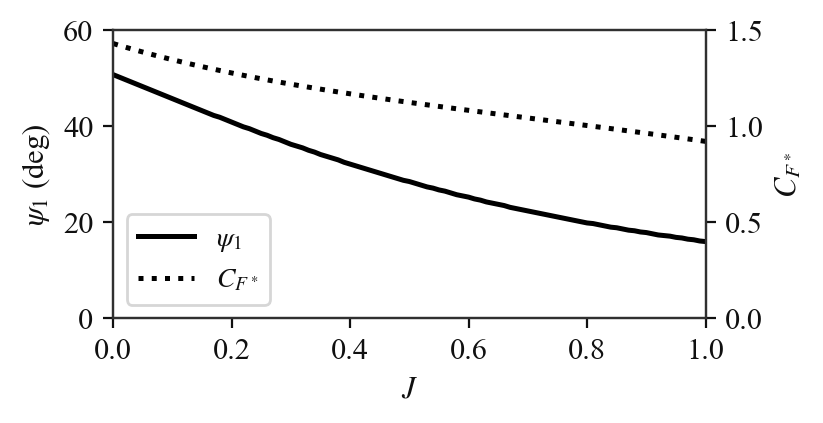
\includegraphics{figures/hover_optimum_J.light.png}
    \caption{Pitch amplitude $\psi_1$ and force coefficient $C_{F^*}$ of
    the continued hover optimum (the point tracked in
    \autoref{fig:cf_J}) as functions of advance ratio $J$. The point
    turns from a local maximum into a saddle at $J \approx
    0.46$.}\label{fig:hover_opt_J}
\end{figure}
\begin{figure}[htbp]
    \centering
    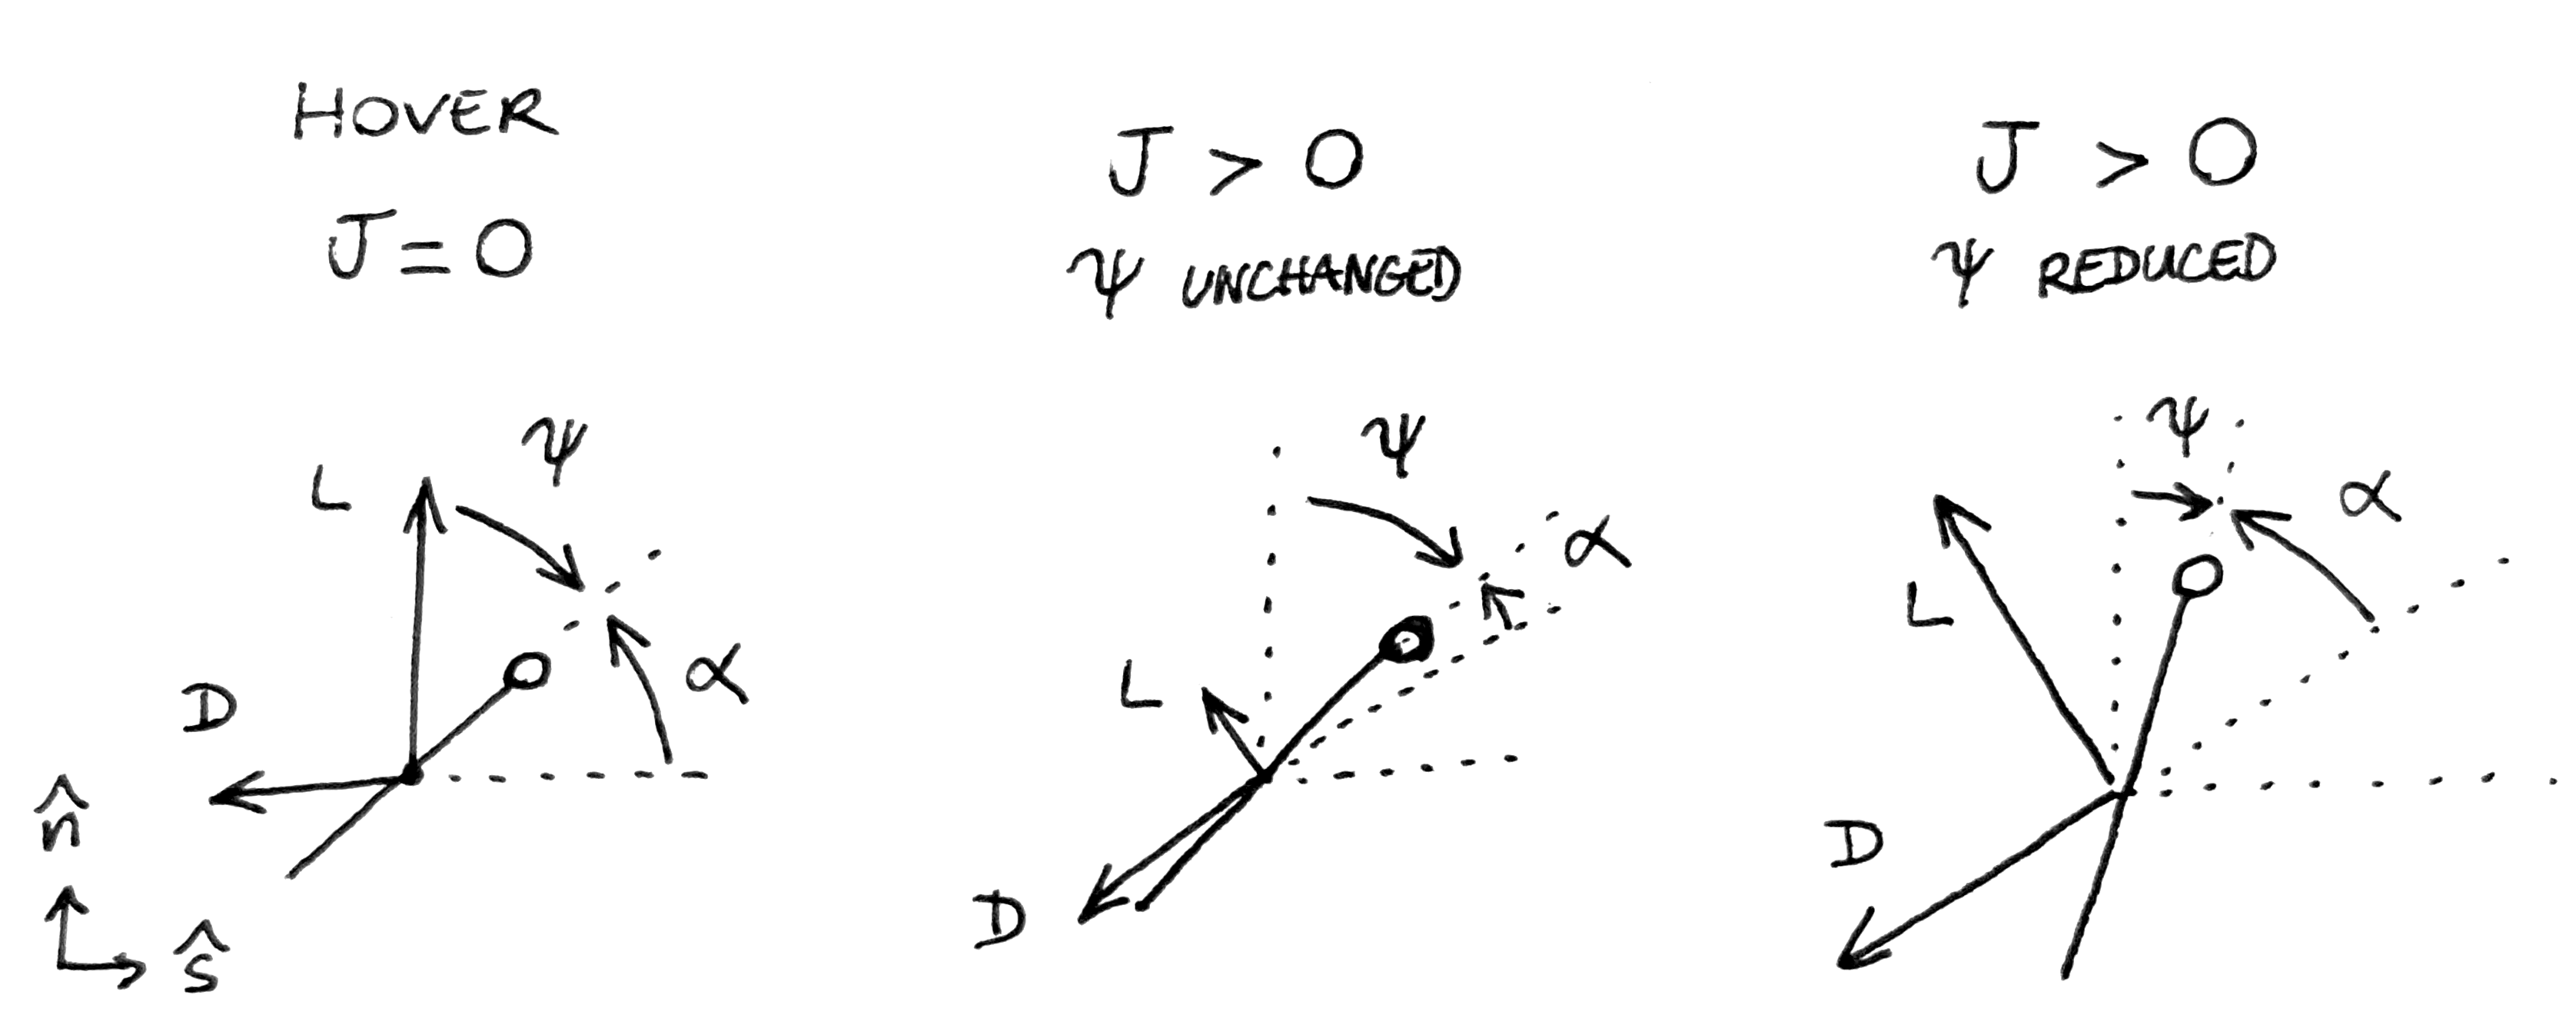
\includegraphics[width=0.85\textwidth]{figures/psi1-decrease-mechanism.png}
    \caption{Illustration of the $\psi$ reduction mechanism for maximizing stroke-plane-normal force as $J$ increases.}\label{fig:psi1-decrease}
\end{figure}

Finally, \autoref{fig:beta_vs_psi0_J} shows $\beta$
as a function of $\psi_0$ for $J$ from 0 to 1.
Specifically, since $\beta$ now depends on $\psi_1$
in addition to $\psi_0$ (see \autoref{eq:beta-general}),
each line is obtained using the $\psi_1$ value
adapted to the value of $J$ (as shown in \autoref{fig:cf_J}).
As $J$ is increased, there is a clear steepening of
the slope around $\psi_0 = 0$,
meaning control authority is significantly increased.
This would tend to suggest that any gain
associated with the control variable $\psi_0$ may
need to adapt based on the current $J$.
\begin{figure}[htbp]
    \centering
    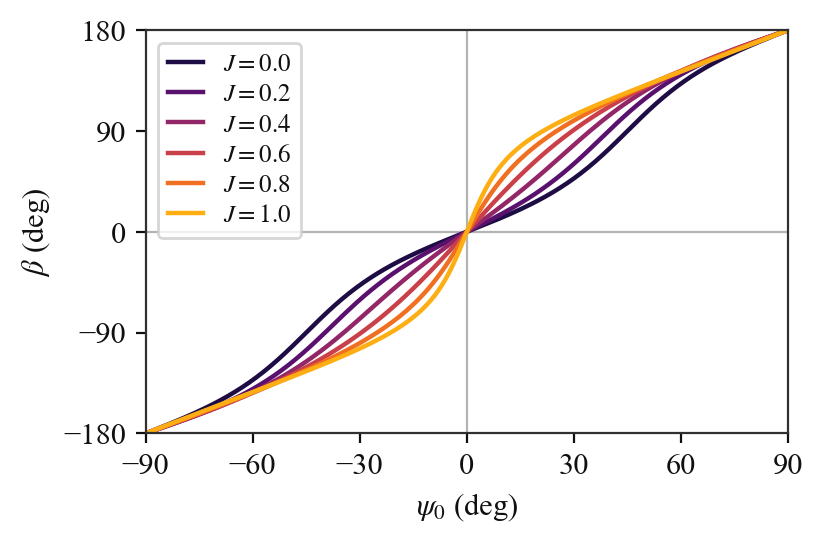
\includegraphics{figures/force_direction_J.light.png}
    \caption{Effect of $\psi_0$ on the force direction angle $\beta$ for
    increasing advance ratio $J$, at $\delta_0 = 90^\circ$ and with
    $\psi_1$ set, for each $J$, to the continued-optimum value of
    \autoref{fig:hover_opt_J}. Unlike in the hover case, $\beta$ depends
    on $\psi_1$ when $J > 0$.}\label{fig:beta_vs_psi0_J}
\end{figure}

We conclude this analytical section by
summarizing the kinematic parameters for the general case,
in \autoref{tab:param-general}. Since there is no requirement
for steady flight like in hover, no specific values for the control
variables $s_0^*$ and $\psi_0$ are prescribed, however the relevant
variables that would inform the choice of the values are still listed.
\begin{table}[htbp]
  \centering
  \caption{Wing kinematic parameters (general case)}
  \label{tab:param-general}
  \begin{tabular}{llr}
    \toprule
    Parameter & Value & Variables \\
    \midrule
    $s_0^*$ & --- & $\frac{A^*}{m^*} \quad \omega^* \quad \gamma \quad C_{L,0} \quad \Delta C_D \quad \bar{C}_D \quad J$ \\
    $\psi_0$ & --- & $\gamma \quad C_{L,0} \quad \Delta C_D \quad \bar{C}_D \quad J$\\
    $\psi_1$ & $\psi_1^\text{opt}(J)$ & $J \quad C_{L,0} \quad \Delta C_D$ \\
    $\delta_0$ & $90^\circ$ & None \\
    \bottomrule
  \end{tabular}
\end{table}

\subsection{Control Strategy}

\section{Results}\label{sec:results}

\subsection{Hover}

\subsection{Prescribed Trajectory}

\subsection{Prey Pursuit}

\FloatBarrier
\bibliographystyle{unsrtnat}
\bibliography{references}

\end{document}
